%%%%%%%%%%%%  Generated using docx2latex.com  %%%%%%%%%%%%%%

%%%%%%%%%%%%  v2.0.0-beta  %%%%%%%%%%%%%%

\documentclass[12pt]{article}
\usepackage{amsmath}
\usepackage{latexsym}
\usepackage{amsfonts}
\usepackage[normalem]{ulem}
\usepackage{array}
\usepackage{amssymb}
\usepackage{graphicx}
\usepackage[backend=biber,
style=numeric,
sorting=none,
isbn=false,
doi=false,
url=false,
]{biblatex}\addbibresource{bibliography.bib}

\usepackage{subfig}
\usepackage{wrapfig}
\usepackage{wasysym}
\usepackage{enumitem}
\usepackage{adjustbox}
\usepackage{ragged2e}
\usepackage[svgnames,table]{xcolor}
\usepackage{tikz}
\usepackage{longtable}
\usepackage{changepage}
\usepackage{setspace}
\usepackage{hhline}
\usepackage{multicol}
\usepackage{tabto}
\usepackage{float}
\usepackage{multirow}
\usepackage{makecell}
\usepackage{fancyhdr}
\usepackage[toc,page]{appendix}
\usepackage[hidelinks]{hyperref}
\usetikzlibrary{shapes.symbols,shapes.geometric,shadows,arrows.meta}
\tikzset{>={Latex[width=1.5mm,length=2mm]}}
\usepackage{flowchart}\usepackage[paperheight=11.69in,paperwidth=8.27in,left=1.18in,right=1.18in,top=0.98in,bottom=0.98in,headheight=1in]{geometry}
\usepackage[utf8]{inputenc}
\usepackage[T1]{fontenc}
\TabPositions{0.49in,0.98in,1.47in,1.96in,2.45in,2.94in,3.43in,3.92in,4.41in,4.9in,5.39in,5.88in,}

\urlstyle{same}


 %%%%%%%%%%%%  Set Depths for Sections  %%%%%%%%%%%%%%

% 1) Section
% 1.1) SubSection
% 1.1.1) SubSubSection
% 1.1.1.1) Paragraph
% 1.1.1.1.1) Subparagraph


\setcounter{tocdepth}{5}
\setcounter{secnumdepth}{5}


 %%%%%%%%%%%%  Set Depths for Nested Lists created by \begin{enumerate}  %%%%%%%%%%%%%%


\setlistdepth{9}
\renewlist{enumerate}{enumerate}{9}
		\setlist[enumerate,1]{label=\arabic*)}
		\setlist[enumerate,2]{label=\alph*)}
		\setlist[enumerate,3]{label=(\roman*)}
		\setlist[enumerate,4]{label=(\arabic*)}
		\setlist[enumerate,5]{label=(\Alph*)}
		\setlist[enumerate,6]{label=(\Roman*)}
		\setlist[enumerate,7]{label=\arabic*}
		\setlist[enumerate,8]{label=\alph*}
		\setlist[enumerate,9]{label=\roman*}

\renewlist{itemize}{itemize}{9}
		\setlist[itemize]{label=$\cdot$}
		\setlist[itemize,1]{label=\textbullet}
		\setlist[itemize,2]{label=$\circ$}
		\setlist[itemize,3]{label=$\ast$}
		\setlist[itemize,4]{label=$\dagger$}
		\setlist[itemize,5]{label=$\triangleright$}
		\setlist[itemize,6]{label=$\bigstar$}
		\setlist[itemize,7]{label=$\blacklozenge$}
		\setlist[itemize,8]{label=$\prime$}

\setlength{\topsep}{0pt}\setlength{\parindent}{0pt}
\renewcommand{\arraystretch}{1.3}


%%%%%%%%%%%%%%%%%%%% Document code starts here %%%%%%%%%%%%%%%%%%%%



\begin{document}
\setlength{\parskip}{14.04pt}
\textbf{UNIVERSIDAD POLITÉCNICA DE LA ZONA METROPOLITANA DE GUADALAJARA}\par

\textbf{\textcolor[HTML]{ED1C24}{GIRO DE MOTOR CORRIENTE DIRECTA}}\par

\textbf{Por: Jesús David Esparza Cabrera}\par

\textbf{Grado y grupo: 4-B}\par



%%%%%%%%%%%%%%%%%%%% Figure/Image No: 1 starts here %%%%%%%%%%%%%%%%%%%%

\begin{figure}[H]
	\begin{Center}
		
\includegraphics[width=2.71in,height=2.74in]{./media/image1.png}
	\end{Center}
\end{figure}


%%%%%%%%%%%%%%%%%%%% Figure/Image No: 1 Ends here %%%%%%%%%%%%%%%%%%%%

\par


\vspace{\baselineskip}

\vspace{\baselineskip}

\vspace{\baselineskip}

\vspace{\baselineskip}

\vspace{\baselineskip}

\vspace{\baselineskip}

\vspace{\baselineskip}
Un \textbf{motor eléctrico} es una \href{http://es.wikipedia.org/wiki/Máquina_eléctrica}{máquina eléctrica} que transforma \href{http://es.wikipedia.org/wiki/Energía_eléctrica}{energía eléctrica} en \href{http://es.wikipedia.org/wiki/Energía_mecánica}{energía mecánica} por medio de interacciones \href{http://es.wikipedia.org/wiki/Electromagnetismo}{electromagnéticas}. Algunos de los motores eléctricos son reversibles, pueden transformar energía mecánica en energía eléctrica funcionando como \href{http://es.wikipedia.org/wiki/Generador_eléctrico}{generadores}. Los motores eléctricos de tracción usados en locomotoras realizan a menudo ambas tareas, si se los equipa con \href{http://es.wikipedia.org/wiki/Freno_regenerativo}{frenos regenerativos}.\par

Son ampliamente utilizados en instalaciones industriales, comerciales y de particulares. Pueden funcionar conectados a una \href{http://es.wikipedia.org/wiki/Red_de_suministro_eléctrico}{red de suministro eléctrico} o a \href{http://es.wikipedia.org/wiki/Batería_eléctrica}{baterías}. Así, en \href{http://es.wikipedia.org/wiki/Automóvil}{automóviles} se están empezando a utilizar en \href{http://es.wikipedia.org/wiki/Vehículo_híbrido}{vehículos híbridos} para aprovechar las ventajas de ambos.\par

\begin{enumerate}
	\item  Principio de funcionamiento\par

Los motores de \href{http://es.wikipedia.org/wiki/Corriente_alterna}{corriente alterna} y los motores de \href{http://es.wikipedia.org/wiki/Corriente_continua}{corriente continua} se basan en el mismo principio de funcionamiento, el cuál establece que si un conductor por el cual circula una \href{http://es.wikipedia.org/wiki/Corriente_eléctrica}{corriente eléctrica} se encuentra dentro de la acción de un \href{http://es.wikipedia.org/wiki/Campo_magnético}{campo magnético}, éste tiende a desplazarse perpendicularmente a las líneas de acción del \href{http://es.wikipedia.org/wiki/Campo_magnético}{campo magnético}.\par

El conductor tiende a funcionar como un \href{http://es.wikipedia.org/wiki/Electroimán}{electroimán} debido a la \href{http://es.wikipedia.org/wiki/Corriente_eléctrica}{corriente eléctrica} que circula por el mismo adquiriendo de esta manera propiedades magnéticas, que provocan, debido a la interacción con los polos ubicados en el estator, el movimiento circular que se observa en el rotor del motor.\par

Partiendo del hecho de que cuando pasa corriente eléctrica por un conductor se produce un \href{http://es.wikipedia.org/wiki/Campo_magnético}{campo magnético}, además si lo ponemos dentro de la acción de un \href{http://es.wikipedia.org/wiki/Campo_magnético}{campo magnético} potente, el producto de la interacción de ambos campos magnéticos hace que el conductor tienda a desplazarse produciendo así la energía mecánica. Dicha \href{http://es.wikipedia.org/wiki/Energía}{energía} es comunicada al exterior mediante un dispositivo llamado flecha.\par



%%%%%%%%%%%%%%%%%%%% Figure/Image No: 2 starts here %%%%%%%%%%%%%%%%%%%%

\begin{figure}[H]
	\begin{Center}
		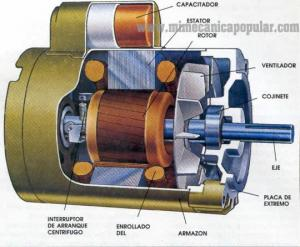
\includegraphics[width=3.13in,height=2.57in]{./media/image2.jpeg}
	\end{Center}
\end{figure}


%%%%%%%%%%%%%%%%%%%% Figure/Image No: 2 Ends here %%%%%%%%%%%%%%%%%%%%

\par

	\item Ventajas\par

En diversas circunstancias presenta muchas ventajas respecto a los \href{http://es.wikipedia.org/wiki/Motor_de_combustión}{motores de combustión}:\par

\setlength{\parskip}{0.0pt}
\begin{itemize}
	\item A igual \href{http://es.wikipedia.org/wiki/Potencia}{potencia}, su tamaño y peso son más reducidos. \par

	\item Se pueden construir de cualquier tamaño. \par

	\item Tiene un \href{http://es.wikipedia.org/wiki/Par_de_giro}{par de giro} elevado y, según el tipo de motor, prácticamente constante. \par

	\item Su \href{http://es.wikipedia.org/wiki/Rendimiento}{rendimiento} es muy elevado (típicamente en torno al 75$\%$ , aumentando el mismo a medida que se incrementa la potencia de la máquina). \par

\setlength{\parskip}{14.04pt}
	\item Este tipo de motores no emite contaminantes, aunque en la \href{http://es.wikipedia.org/wiki/Generación_de_energía_eléctrica}{generación de energía eléctrica} de la mayoría de las redes de suministro se emiten contaminantes. 
\end{itemize}\par

	\item Motores de corriente continua\par


\vspace{\baselineskip}


%%%%%%%%%%%%%%%%%%%% Figure/Image No: 3 starts here %%%%%%%%%%%%%%%%%%%%


\begin{figure}[H]	\begin{subfigure}		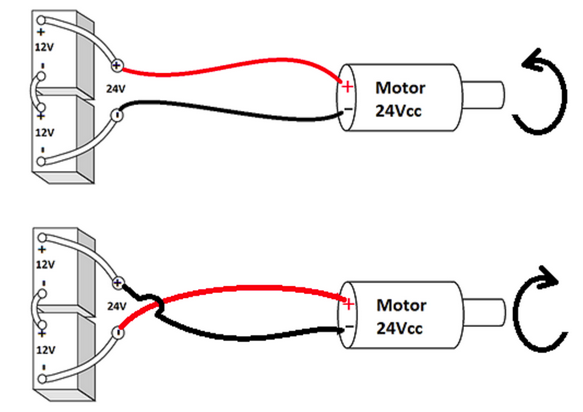
\includegraphics[width=0.45\textwidth]{./media/image3.png}
	\end{subfigure}
~	\begin{subfigure}		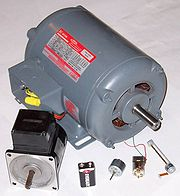
\includegraphics[width=0.45\textwidth]{./media/image4.jpeg}
	\end{subfigure}
~
\end{figure}


%%%%%%%%%%%%%%%%%%%% Figure/Image No: 3 Ends here %%%%%%%%%%%%%%%%%%%%

 \par


\vspace{\baselineskip}
\textbf{\textcolor[HTML]{33002B}{Diversos motores eléctricos}}\par

Los motores de \href{http://es.wikipedia.org/wiki/Corriente_continua}{corriente continua} se clasifican según la forma como estén conectados, en:\par

\setlength{\parskip}{0.0pt}
\begin{itemize}
	\item \href{http://es.wikipedia.org/wiki/Motor_serie}{Motor serie} \par

	\item \href{http://es.wikipedia.org/wiki/Motor_compound}{Motor compound} \par

	\item \href{http://es.wikipedia.org/wiki/Motor_shunt}{Motor shunt} \par

\setlength{\parskip}{14.04pt}
	\item \href{http://es.wikipedia.org/wiki/Motor_eléctrico_sin_escobillas}{Motor eléctrico sin escobillas} 
\end{itemize}\par

Además de los anteriores, existen otros tipos que son utilizados en electrónica:\par

\setlength{\parskip}{0.0pt}
\begin{itemize}
	\item \href{http://es.wikipedia.org/wiki/Motor_paso_a_paso}{Motor paso a paso} \par

	\item \href{http://es.wikipedia.org/wiki/Servomotor}{Servomotor} \par

\setlength{\parskip}{14.04pt}
	\item \href{http://es.wikipedia.org/wiki/Motor_sin_núcleo}{Motor sin núcleo} 
\end{itemize}\par

	\item Conclusión
\end{enumerate}\par

Un motor eléctrico de corriente continua es esencialmente una máquina que convierte energía eléctrica en \href{https://www.monografias.com/trabajos15/kinesiologia-biomecanica/kinesiologia-biomecanica.shtml}{movimiento} o \href{https://www.monografias.com/trabajos34/el-trabajo/el-trabajo.shtml}{trabajo} mecánico, a través de \href{https://www.monografias.com/trabajos14/medios-comunicacion/medios-comunicacion.shtml}{medios} electromagnéticos, que para funcionar se vale de las fuerzas de atracción y repulsión que existen entre los polos.\par

El motor de corriente continua está compuesto de 2 piezas fundamentales:\par

- Rotor\par

- Estator\par

Dentro de éstas se ubican los demás componentes como:\par

- Escobillas y porta escobillas\par

- Colector\par

- Eje\par

- Núcleo y devanado del rotor\par

- Imán Permanente\par

- Armazón\par

-Tapas o campana\par

Los motores de corriente continua son de menos utilización que los motores de corriente alterna en el área industrial, debido que los motores de corriente alterna se alimentan con los \href{https://www.monografias.com/trabajos11/teosis/teosis.shtml}{sistemas} de \href{https://www.monografias.com/trabajos11/travent/travent.shtml}{distribución} de energías "normales".\par

{\fontsize{15pt}{18.0pt}\selectfont \textbf{Bibliografía}\par}\par

\href{http://perso.wanadoo.es/luis_ju/ebasica2/mcc_01.html}{http://perso.wanadoo.es/luis\_ju/ebasica2/mcc\_01.html}\par

\setlength{\parskip}{6.96pt}
\href{http://www.unicrom.com/Tut_MotorCC.asp}{http://www.unicrom.com/Tut\_MotorCC.asp}\par


\printbibliography
\end{document}